\section{Experimental and theoretical input}
\label{sec:expdata}

The NNPDF3.1 PDF sets include a wealth of new experimental data.  We
have augmented our dataset with improved determinations of observables
already included in NNPDF 3.0 (such as $W$ and $Z$ rapidity
distributions) as well as two new process: top quark differential
distributions, and the $Z$ transverse momentum distribution, which is
include for the first time in a global PDF determination.

In this Section we discuss the NNPDF3.1 dataset in detail. After a
general overview, each observable 
will be examined: we describe the individual measurements, and 
address specific theoretical and phenomenological issues related to
their inclusion, particularly in relation to the use of recent NNLO results.

In NNPDF3.1 only LHC data from Run I, taken at centre-of-mass
energies of 2.76~TeV, 7~TeV and 8~TeV (with one single exception), are included. The more recent 13~TeV
dataset is reserved for phenomenological comparison purposes in Sect.~\ref{sec:pheno}.
%
Available and upcoming LHC Run II data at 13~TeV will be part of future NNPDF releases.

\subsection{Experimental data: general overview}

The NNPDF3.0 global analysis involved data from deep-inelastic scattering (DIS) experiments, fixed-target Drell-Yan data, and
collider measurements from the Tevatron and LHC.
The fixed-target and collider DIS datasets included measurements from NMC~\cite{Arneodo:1996kd,Arneodo:1996qe}, 
BCDMS~\cite{bcdms1,bcdms2} and SLAC~\cite{Whitlow:1991uw}; the combined HERA-I 
inclusive structure function dataset~\cite{Aaron:2009aa} and HERA-II inclusive measurements
from H1 and ZEUS~\cite{Aaron:2012qi,Collaboration:2010ry,ZEUS:2012bx,Collaboration:2010xc};
the HERA combined measurements of the charm production cross-section $\sigma_{c}^{\rm NC}$~\cite{Abramowicz:1900rp};
CHORUS inclusive neutrino DIS~\cite{Onengut:2005kv}, and NuTeV dimuon production 
data~\cite{Goncharov:2001qe,MasonPhD}.
%
From the Tevatron, CDF~\cite{Aaltonen:2010zza} and D0~\cite{Abazov:2007jy} $Z$ rapidity distributions; and
CDF~\cite{Aaltonen:2008eq} Run-II one-jet inclusive cross-sections were used. Constraints from fixed-target Drell-Yan came from the 
E605~\cite{Moreno:1990sf} and E866~\cite{Webb:2003ps,Webb:2003bj,Towell:2001nh} experiments. 
%
LHC measurements included electroweak boson production data from ATLAS~\cite{Aad:2011dm,Aad:2013iua,Aad:2011fp}, 
CMS~\cite{Chatrchyan:2012xt,Chatrchyan:2013mza,Chatrchyan:2013tia} and LHCb~\cite{Aaij:2012vn,Aaij:2012mda};
one-jet inclusive cross-sections from ATLAS~\cite{Aad:2011fc,Aad:2013lpa} and CMS~\cite{Chatrchyan:2012bja};
the differential distributions for $W$ production in association with charm quarks from CMS~\cite{Chatrchyan:2013uja};
and total cross-section measurements for top quark pair production data from ATLAS and CMS at 7 and 8~TeV~\cite{ATLAS:2012aa,ATLAS:2011xha,TheATLAScollaboration:2013dja, Chatrchyan:2013faa,Chatrchyan:2012bra,Chatrchyan:2012ria}.

For NNPDF3.1 we have made a number of improvements to the NNPDF3.0
dataset. Firstly we  have included the final
datasets for several experiments which have now concluded, replacing superseded data in the NNPDF3.0 analysis.
%
The HERA-I data and the H1 and ZEUS HERA-II inclusive structure functions have been replaced by the final 
HERA combination~\cite{Abramowicz:2015mha}.
%
%
The HERA dataset has also been enlarged by the inclusion of H1 and ZEUS measurements of the 
bottom structure function $F_2^b(x,Q^2)$~\cite{Aaron:2009af,Abramowicz:2014zub}, which may prove useful in 
specific applications such as in the determination of the bottom quark mass $m_b$.
%
In order to perform dedicated studies of the charm content of the
proton, we have constructed a PDF set also 
including the EMC measurements of charm structure functions at
large-$x$~\cite{Aubert:1982tt}, which 
will be discussed in Sect.~\ref{sec:phenocharm}. However, these measurements are not included in the standard dataset.
%
The legacy $W$ lepton asymmetries from D0 using the complete Tevatron luminosity, both in the electron~\cite{D0:2014kma}
and in the muon~\cite{Abazov:2013rja} channels have been added.
%
These precise weak gauge boson production measurements provide important information on the quark flavor separation at large-$x$, 
as demonstrated in~\cite{Camarda:2015zba}.

Aside from the updated legacy datsets, in NNPDF3.1 a large number of recent measurements from ATLAS, CMS and LHCb are included.
%
For ATLAS, we now include the $Z$ boson $(p_T^Z,y_Z)$ and $(p_T^Z,M_{ll})$ double differential distributions measured at 8~TeV~\cite{Aad:2015auj}; the inclusive $W^+$, $W^-$ and $Z$ rapidity distributions at 
7~TeV from the 2011 dataset~\cite{Aaboud:2016btc}, the top-quark pair production normalized $y_t$ distribution at 8~TeV~\cite{Aad:2015mbv}; total cross-sections for top quark pair production at 7, 8 and 13~TeV~\cite{Aad:2014kva,Aaboud:2016pbd}; inclusive jet cross-sections at 7~TeV from the 2011 dataset~\cite{Aad:2014vwa}; and 
finally low mass Drell-Yan $M_{ll}$ distributions at 7~TeV from the 2010 run~\cite{Aad:2014qja}. The transverse momentum 
spectrum at 7~TeV (2011 dataset)~\cite{Aad:2014xaa} will be studied in Sec.~\ref{sec:impactzpt} but it is not included in the default 
set. The total top cross-section is the only data point at 13~TeV which
is included.
For CMS, NNPDF3.1 includes the $W^+$ and $W^-$ rapidity distributions at 8~TeV~\cite{Khachatryan:2016pev},
together with their cross-correlations; the inclusive jet production
cross-sections at 2.76~TeV~\cite{Khachatryan:2015luy};
top-quark pair production normalized $y_{t\bar{t}}$ distributions at 8~TeV~\cite{Khachatryan:2015oqa}, total inclusive $t\bar{t}$ cross-sections at 7, 8
and 13~TeV~\cite{Khachatryan:2016mqs}; the distribution of the
$Z$ boson double differentially in $(p_T,y_Z)$ at 8~TeV~\cite{Khachatryan:2015oaa}. The double-differential
distributions $(y_{ll},M_{ll})$ in Drell-Yan production at 8~TeV~\cite{CMS:2014jea} will be studied in
Sect.~\ref{sec:cms8tevimpact} below, but it is not included in the default
PDF determination.
For LHCb, NNPDF3.1 includes the
complete 7 and 8~TeV measurements of inclusive $W$ and $Z$
production in the muon
channel~\cite{Aaij:2015gna,Aaij:2015zlq}, which supersedes all previous
measurements in the same final state.

An overview of the data included in NNPDF3.1 is presented in
Tables~\ref{tab:completedataset},~\ref{tab:completedataset2},
and~\ref{tab:completedataset3}, for the DIS structure function data,
the fixed target and Tevatron Drell-Yan experiments, and the LHC
datasets, respectively.
%
For each dataset we indicate the corresponding published reference, the number
of data points in the NLO/NNLO PDF determinations 
before and after (in parenthesis) kinematic cuts, the kinematic
range covered in the relevant variables after cuts, and the code used
to compute the NLO and NNLO results.
%
Datasets included 
for the first time in NNPDF3.1 are flagged with an asterisk. The
datasets not used for the default determination are in brackets. 
The total number of data points for the default
PDF determination 
is $4175/4295/4285$ at LO/NLO/NNLO.

%%%%%%%%%%%%%%%%%%%%%%%%%%%%%%%
%%%%%%%%%%%%%%%%%%%%%%%%%%%%%%%%%%%%%%%%%%%%%%%%%%%%%%%%%%%%%%%%%
%%%%%%%%%%%%%%%%%%%%%%%%%%%%%%%%%%%%%%%%%%%%%%%%%%%%%%%%%%%%%%%%%

\begin{table}
\footnotesize
\begin{centering}
      \renewcommand{\arraystretch}{1.4}
  \begin{tabular}{|c|c|c|c|c|c|c|}
\hline
{Experiment} & Obs. & {Ref.}  & $ N_{\rm \bf dat}$ & $x$ range  & $Q$ range (GeV)  & Theory \tabularnewline
\hline
\hline
\multirow{2}{*}{NMC}
&   $F_2^d/F_2^p$ & \cite{Arneodo:1996kd}&   260 (121/121) & $ 0.012\le x \le 0.68$
& $ 2.1 \le Q \le 10 $  &\multirow{2}{*}{\tt APFEL}\tabularnewline
&   $\sigma^{\rm NC,p}$ & \cite{Arneodo:1996qe} & 292 (204/204) &
$0.012 \le x \le 0.50$ & $ 1.8 \le Q \le 7.9 $  &  \tabularnewline
\hline
\multirow{2}{*}{SLAC} &   $F_2^p$ & \cite{Whitlow:1991uw} &  211 (33/33)
& $ 0.14\le x \le 0.55$  &
$ 1.9 \le Q \le 4.4 $  & \multirow{2}{*}{\tt APFEL}\tabularnewline
&   $F_2^d$ & \cite{Whitlow:1991uw}& 211 (34/34) &
$ 0.14 \le x \le 0.55 $ & $ 1.9\le Q \le 4.4 $  & \tabularnewline
\hline
\multirow{2}{*}{BCDMS} &   $F_2^p$ & \cite{bcdms1}&  351 (333/333) & $0.07 \le x \le 0.75$ & $
2.7\le Q \le 15.1 $  &
\multirow{2}{*}{\tt APFEL}\tabularnewline
&   $F_2^d$ & \cite{bcdms2}&  254 (248/248) & $0.07 \le x \le 0.75$ & $ 3.0\le  Q \le
15.1$  & \tabularnewline
\hline
\multirow{2}{*}{CHORUS} &  $\sigma^{\rm CC,\nu}$  & \cite{Onengut:2005kv} & 607 (416/416) &
$0.045 \le x \le 0.65 $  &
$ 1.9\le Q \le 9.8 $  &
\multirow{2}{*}{\tt APFEL} \tabularnewline
&   $\sigma^{\rm CC,\bar{\nu}}$ & \cite{Onengut:2005kv} & 607 (416/416)  & $0.045 \le x \le 0.65$  &
$ 1.9 \le Q \le 9.8 $  & \tabularnewline
\hline
\multirow{2}{*}{NuTeV} &    $\sigma_\nu^{cc}$ & \cite{Goncharov:2001qe,MasonPhD} & 45 (39/39)
&$ 0.02 \le x \le 0.33 $ &
$ 2.0 \le Q \le 10.8  $ 
& \multirow{2}{*}{\tt APFEL} \tabularnewline
&   $\sigma_{\bar{\nu}}^{cc}$ & \cite{Goncharov:2001qe,MasonPhD} & 45 (37/37) &
$ 0.02 \le x \le 0.21$&
$ 1.9 \le Q \le 8.3 $ 
&\tabularnewline
\hline
\multirow{3}{*}{HERA}  &  $\sigma_{\rm NC,CC}^{p}$ {\bf (*)} & \cite{Abramowicz:2015mha}
&  1306 (1145/1145)  & $4\cdot 10^{-5}\le x \le 0.65$ & $ 1.87 \le Q \le 223 $   & \multirow{3}{*}{\tt APFEL}
 \tabularnewline
  & $\sigma_{\rm NC}^{c}$    & \cite{Abramowicz:1900rp} & 52 (47/37) & $7 \cdot 10^{-5} \le x \le 0.05$  & $2.2 \le Q \le 45$  &
 \tabularnewline
 &  $F_2^b$   {\bf (*)} & \cite{Aaron:2009af,Abramowicz:2014zub} & 29 (29/29) & $ 2\cdot 10^{-4}\le x \le
 0.5 $ & $ 2.2 \le Q \le 45$  &
 \tabularnewline
 \hline
 EMC
 &   [ $F_2^c$ ] {\bf (*)}  & \cite{Aubert:1982tt} & 21 (16/16) &$0.014\le x \le 0.44$  & $2.1 \le Q \le 8.8 $ & \tt APFEL
 \tabularnewline
  \hline
\end{tabular}
\par\end{centering}
\caption{\small Deep-inelastic scattering
data included in  NNPDF3.1. The EMC $F_2^c$ data are in brackets because
they are only included in a dedicated set but not in the default dataset.
New datasets, not included in NNPDF3.0, are
denoted {\bf (*)}. 
The kinematic range covered in each variable is given after cuts are applied. 
The total number of DIS data points after cuts is 
$3102/3092$ for the NLO/NNLO PDF determinations (not including the EMC $F_2^c$ data).
\label{tab:completedataset}
}
\end{table}
%%%%%%%%%%%%%%%%%%%%%%%%%%%%%%%%%%%%%%%%%%%%%%%%%%%%%%%%%%%%%%%%%%%%%%%%%
%%%%%%%%%%%%%%%%%%%%%%%%%%%%%%%%%%%%%%%%%%%%%%%%%%%%%%%%%%%%%%%%%%%%%%%%%

\begin{table}
\footnotesize
\begin{centering}
    \renewcommand{\arraystretch}{1.4}
\begin{tabular}{|c|c|c|c|c|c|c|}
\hline
{Exp.} & Obs. & {Ref.}  & $ N_{\rm \bf dat}$ & Kin$_1$  & Kin$_2$ (GeV) & Theory \tabularnewline
\hline
\hline
\multirow{2}{*}{E866} &   $\sigma_{\rm DY}^d/\sigma_{\rm DY}^p$ & \cite{Towell:2001nh} & 15 (15/15)
& 0.07 $\le y_{ll}\le 1.53$ &
$ 4.6 \le M_{ll}\le 12.9 $  & {\tt APFEL+Vrap}\tabularnewline
&  $\sigma_{\rm DY}^p$ & \cite{Webb:2003ps,Webb:2003bj} & 184 (89/89) & $0 \le y_{ll}\le 1.36 $ &
$  4.5 \le M_{ll}\le 8.5 $  &{\tt APFEL+Vrap} \tabularnewline
 \hline
 E605 & $\sigma_{\rm DY}^p$ &  \cite{Moreno:1990sf} & 119 (85/85) & $ -0.2 \le y_{ll}\le 0.4$ &
 $ 7.1 \le M_{ll}\le 10.9 $  & {\tt APFEL+Vrap} \tabularnewline
 \hline
\multirow{2}{*}{CDF} &   $d\sigma_Z/dy_Z$ & \cite{Aaltonen:2010zza}&  29 (29/29)  & $ 0 \le y_{ll}\le 2.9 $  & $66 \le M_{ll}\le 116$   &{\tt Sherpa+Vrap} \tabularnewline
&  $k_t$ incl jets & \cite{Abulencia:2007ez} & 76 (76/76) & $ 0\le y_{\rm jet}\le 1.9$  &
 $ 58 \le p_T^{\rm jet}\le 613$  &{\tt NLOjet++} \tabularnewline
\hline
\multirow{3}{*}{D0}   &   $d\sigma_Z/dy_Z$ &  \cite{Abazov:2007jy}  & 28 (28/28) & $0 \le y_{ll}\le 2.8 $ &
 $66 \le M_{ll}\le 116$ & {\tt Sherpa+Vrap}\tabularnewline
&   $W$ electron asy {\bf (*)}  & \cite{D0:2014kma}  & 13  (13/8) &  $0 \le y_{e}\le 2.9 $& $Q=M_W$  &{\tt MCFM}+{\tt FEWZ}\tabularnewline
 &   $W$ muon asy {\bf (*)}  & \cite{Abazov:2013rja}  &  10 (10/9)   & $0 \le y_{\mu}\le 1.9 $ & $Q=M_W$ & {\tt MCFM}+{\tt FEWZ}\tabularnewline
  \hline
\end{tabular}
\par\end{centering}
\caption{\small Same as Table~\ref{tab:completedataset}
  for the Tevatron fixed-target Drell-Yan  and $W$, $Z$ and jet collider
  data. The total number of Tevatron data points after cuts is $345/339$ 
for NLO/NNLO fits.
\label{tab:completedataset2}
}
\end{table}
%%%%%%%%%%%%%%%%%%%%%%%%%%%%%%%%%%%%%%%%%%%%%%%%%%%%%%%%%%%%%%%%%%%%%%%%%
%%%%%%%%%%%%%%%%%%%%%%%%%%%%%%%%%%%%%%%%%%%%%%%%%%%%%%%%%%%%%%%%%%%%%%%%%

%%%%%%%%%%%%%%%%%%%%%%%%%%%%%%%%%%%%%%%%%%%%%%%%%%%%%%%%%%%%%%%%%%%%%%%%%
%%%%%%%%%%%%%%%%%%%%%%%%%%%%%%%%%%%%%%%%%%%%%%%%%%%%%%%%%%%%%%%%%%%%%%%%%
\begin{table}[ht]
\scriptsize
\begin{centering}
   \renewcommand{\arraystretch}{1.4}
\begin{tabular}{|c|c|c|c|c|c|c|}
  \hline
  {Exp.} & Obs. & {Ref.}  & $ N_{\rm \bf dat}$  & Kin$_1$  &  Kin$_2$ (GeV) & Theory \tabularnewline
\hline
\hline
\multirow{12}{*}{ATLAS} &   $W,Z$ 2010 & \cite{Aad:2011dm}  &  30 (30/30) & $ 0 \le |\eta_l| \le 3.2$ & $Q=M_W, M_Z$ &
{\tt MCFM}+{\tt FEWZ}\tabularnewline
&   $W,Z$ 2011 {\bf (*)}  & \cite{Aaboud:2016btc}  & 34 (34/34)   & $0 \le |\eta_l| \le 2.3$   & $Q=M_W, M_Z$ &
{\tt MCFM}+{\tt FEWZ}\tabularnewline
&    high-mass DY 2011 & \cite{Aad:2013iua}  & 11 (5/5) & $0 \le |\eta_l| \le 2.1$ & $ 116 \le M_{ll} \le 1500$  &
{\tt MCFM}+{\tt FEWZ} \tabularnewline
&    low-mass DY 2011 {\bf (*)}   & \cite{Aad:2014qja}  & 6 (4/6)  & $0 \le  |\eta_l| \le 2.1$  & $  14 \le M_{ll} \le 56  $  &
{\tt MCFM}+{\tt FEWZ}
\tabularnewline
&    [$Z$ $p_T$ 7 TeV $\lp p_T^Z,y_Z\rp$]  {\bf (*)}  & \cite{Aad:2014xaa}  & 64 (39/39)  &
$0 \le |y_{Z}| \le 2.5$  &  $30 \le p_T^Z \le 300$   & {\tt MCFM}+NNLO
\tabularnewline
&    $Z$ $p_T$ 8 TeV $\lp p_T^Z,M_{ll}\rp$  {\bf (*)}  & \cite{Aad:2015auj}  & 64 (44/44)  &  $  12 \le M_{ll} \le
150 $  GeV & $30 \le p_T^Z \le 900$  & {\tt MCFM}+NNLO
      \tabularnewline
      &    $Z$ $p_T$ 8 TeV $\lp p_T^Z,y_Z\rp$  {\bf (*)}  & \cite{Aad:2015auj}  & 120 (48/48)  & $   0.0\le |y_{Z}| \le 2.4  $  
        & $   30\le p_{T}^Z \le 150  $  &
          {\tt MCFM}+NNLO
            \tabularnewline
&    7 TeV jets 2010 & \cite{Aad:2011fc}  & 90 (90/90) &
$0 \le |y^{\rm jet}| \le 4.4 $ & $ 25 \le p_T^{\rm jet} \le 1350 $&
{\tt NLOjet++}
\tabularnewline
&      2.76 TeV jets  &  \cite{Aad:2013lpa}  &
59 (59/59) & $0 \le |y^{\rm jet}| \le 4.4$ & $20 \le p_T^{\rm jet} \le 200$ & {\tt NLOjet++}
\tabularnewline
&      7 TeV jets 2011 {\bf (*)}  &  \cite{Aad:2014vwa}  & 140 (31/31)
  & $ 0 \le |y^{\rm jet}| \le 0.5  $ & $108 \le p_T^{\rm jet} \le 1760 $ & {\tt NLOjet++}
\tabularnewline
  &    $\sigma_{\rm tot}(t\bar{t})$  & \cite{Aad:2014kva,Aaboud:2016pbd}& 
3 (3/3) & - & $Q=m_t$ & {\tt top++} \tabularnewline
 &    $(1/\sigma_{t\bar{t}})d\sigma(t\bar{t})/y_t$  {\bf (*)}   & \cite{Aad:2015mbv}& 
10 (10/10)  & $0<|y_t|<2.5$ & $Q=m_t$ & {\tt Sherpa}+NNLO \tabularnewline
 \hline
 \hline
\multirow{12}{*}{CMS} &   $W$ electron asy & \cite{Chatrchyan:2012xt}  &  11 (11/11) &
$0 \le |\eta_{\rm e}| \le 2.4  $ & $Q=M_W$  & {\tt MCFM}+{\tt FEWZ} \tabularnewline
 &   $W$ muon asy  & \cite{Chatrchyan:2013mza}&   11 (11/11) & 
$0 \le |\eta_{\mu}| \le 2.4  $  & $Q=M_W$ & {\tt MCFM}+{\tt FEWZ} \tabularnewline
&    $W+c$ total  & \cite{Chatrchyan:2013uja}& 5 (5/0) &  $0 \le |\eta_l| \le 2.1$ &
$Q=M_W$  & {\tt MCFM}
\tabularnewline
&    $W+c$ ratio  & \cite{Chatrchyan:2013uja}&  5 (5/0) & $0 \le |\eta_l| \le 2.1$ &
$Q=M_W$
& {\tt MCFM}
\tabularnewline
&   2D DY 2011 7 TeV    & \cite{Chatrchyan:2013tia} &   124 (88/110) & $0 \le |\eta_{ll}| \le 2.2$  &
$20 \le M_{ll} \le 200$  &  {\tt MCFM}+{\tt FEWZ}
\tabularnewline
&   [2D DY 2012 8 TeV]     & \cite{CMS:2014jea} &   124 (108/108) & $0 \le |\eta_{ll}| \le 2.4$  &
$20 \le M_{ll} \le 1200$  &  {\tt MCFM}+{\tt FEWZ}
\tabularnewline
&   $W^{\pm}$ rap 8 TeV  {\bf (*)}     & \cite{Khachatryan:2016pev} &  22 (22/22)   & $0 \le |\eta_{l}| \le 2.3$  &
$Q=M_W$  &  {\tt MCFM}+{\tt FEWZ}
\tabularnewline
&   $Z$ $p_T$ 8 TeV  {\bf (*)}     & \cite{Khachatryan:2015oaa} & 50 (28/28)    & $ 0.0 \le |y_{Z}| \le 1.6 $  &
$  30 \le p_T^Z \le 170 $   &  {\tt MCFM}+NNLO
\tabularnewline
 &   7 TeV jets 2011     & \cite{Chatrchyan:2012bja}&  133 (133/133) &  
$0 \le |y^{\rm jet}| \le 2.5$ & $114 \le p_T^{\rm jet} \le 2116$   &
{\tt NLOjet++}
\tabularnewline
 &   2.76 TeV jets  {\bf (*)}     & \cite{Khachatryan:2015luy}& 81 (81/81)   &  $0 \le |y_{\rm jet}| \le 2.8$
  & $80 \le p_T^{\rm jet} \le$ 570   & {\tt NLOjet++}
 \tabularnewline
&    $\sigma_{\rm tot}(t\bar{t})$   & \cite{Khachatryan:2016mqs,CMS:2016syx}& 
 3 (3/3) & - & $Q=m_t$ & {\tt top++} \tabularnewline
 &     $(1/\sigma_{t\bar{t}})d\sigma(t\bar{t})/y_{t\bar{t}}$ {\bf (*)}   & \cite{Khachatryan:2015oqa}& 
 10 (10/10)  & $-2.1<y_{t\bar{t}}<2.1$  & $Q=m_t$ & {\tt Sherpa}+NNLO \tabularnewline
 \hline
 \hline
\multirow{4}{*}{LHCb} &    $Z$ rapidity 940 pb  & \cite{Aaij:2012vn} &   9 (9/9) &
$2.0 \le \eta_l \le 4.5$& $Q=M_Z$ &
{\tt MCFM}+{\tt FEWZ} \tabularnewline
&    $Z\to ee$ rapidity 2 fb & \cite{Aaij:2012mda}&  17 (17/17) & $2.0 \le \eta_l \le 4.5$ & $Q=M_Z$  & {\tt MCFM}+{\tt FEWZ}
\tabularnewline
&    $W,Z\to \mu$ 7 TeV {\bf (*)}  & \cite{Aaij:2015gna} & 33 (33/29)  & $2.0 \le \eta_l \le 4.5$
& $Q=M_W,M_Z$ &  {\tt MCFM}+{\tt FEWZ}\tabularnewline
&    $W,Z\to \mu$ 8 TeV {\bf (*)}  & \cite{Aaij:2015zlq}  & 34 (34/30) & $2.0 \le \eta_l \le 4.5$
& $Q=M_W,M_Z$ &  {\tt MCFM}+{\tt FEWZ}  \tabularnewline
 \hline
 \end{tabular}
\par\end{centering}
\caption{\small
Same as Table~\ref{tab:completedataset}, for
ATLAS, CMS and LHCb data from the LHC Run I at
$\sqrt{s}=2.76$~TeV,  $\sqrt{s}=7$~TeV and
$\sqrt{s}=8$~TeV. The ATLAS $7$~TeV $Z$ $p_T$ and CMS 2D DY 2012 are
in  brackets because they are only included in a dedicated study
but not in the default PDF set.
The total number of LHC data points after cuts is $848/854$ 
for NLO/NNLO fits (not including ATLAS $7$~TeV $Z$ $p_T$ and CMS 2D DY 2012).
\label{tab:completedataset3}
}
\end{table}
%%%%%%%%%%%%%%%%%%%%%%%%%%%%%%%%%%%%%%%%%%%%%%%%%%%%%%%%%%%%%%%%%
%%%%%%%%%%%%%%%%%%%%%%%%%%%%%%%%%%%%%%%%%%%%%%%%%%%%%%%%%%%%%%%%%


%%%%%%%%%%%%%%%%%%%%%%%%%%%%%%%

In Fig.~\ref{fig:kin31} we show
the kinematic coverage of the NNPDF3.1 dataset in the $\lp x,Q^2\rp$ plane.
For hadronic data, leading-order kinematics have been assumed for
illustrative purposes, with central rapidity used when rapidity is
integrated over and the plotted value of $Q^2$ set equal to the
factorization scale. It is clear that the new data added in NNPDF3.1
are distributed in a wide range of scales and $x$, 
considerably extending the kinematic reach and coverage of the dataset.


%%%%%%%%%%%%%%
\begin{figure}[t]
\centering
\includegraphics[width=0.80\textwidth]{images/plots/kin31.pdf}
\caption{\small 
  The kinematic coverage of the NNPDF3.1 dataset in the $\lp x,Q^2\rp$
  plane.
  %
 \label{fig:kin31}} 
\end{figure}
%%%%%%%%%%%%%%%%%%

In Table~\ref{eq:tablekincuts} we present
a summary of the kinematic cuts applied to the various processes
included in NNPDF3.1 at NLO and NNLO.
These cuts ensure that only data where theoretical calculations are reliable are
included. Specifically, we always remove from the NLO dataset points
for which the NNLO corrections exceed the statistical
uncertainty. The further cuts collected in
Table~\ref{eq:tablekincuts}, specific to individual datasets,  will be 
described
when discussing each dataset in turn. All computations are performed up
to NNLO in QCD, not including electroweak corrections. We have
checked that with the cuts described in Table~\ref{eq:tablekincuts},
electroweak corrections 
never exceed experimental uncertainties. 

The codes used to perform NLO computations will be discussed in each
subsection below. With the exception of deep-inelastic scattering,
NNLO corrections are implemented by computing at the hadron level the
bin-by-bin ratio of 
the NNLO to NLO prediction with a pre-defined PDF set, and applying
the correction to the NLO computation (see Sect.~2.3 of
Ref.~\cite{Ball:2014uwa}). For all new data included in NNPDF3.1,
the PDF set used for the computation of these
correction factors (often refereed to as $K$-factors, and in
Ref.~\cite{Ball:2014uwa} as $C$-factors) is NNPDF3.0, except for the
CMS~W~rap~8~TeV and ATLAS~W/Z~2011 entries of
Tab.~\ref{tab:completedataset3} for which published {\tt xFitter}
results have been used and
the CMS~2D~DY~2012 data for which MMHT PDFs have been
used~\cite{mmhtpriv} 
(see Sect.~\ref{data:inclusiveWZ} below); the
PDF dependence of the correction factors is much smaller than all
other relevant uncertainties as we will demonstrate explicitly in
Sect.~\ref{sec:topdata} below. 




%%%%%%%%%%%%%%%%%%%%%%%%%%%%%%%%%%%%%%%%%%%%%%%%%%%%%%%%%%%%%%%%%%%%%%%%%%%
\begin{table}[t]
  \begin{center}
    \footnotesize
    \renewcommand{\arraystretch}{1.7}
    \begin{tabular}{|l|c|c|}
\hline
Dataset & NLO & NNLO \\
\hline
\hline
\multirow{2}{*}{DIS structure functions}  & $W^2\ge 12.5$ GeV$^2$ & $W^2\ge 12.5$ GeV$^2$ \\
& $Q^2\ge 3.5$ GeV$^2$ & $Q^2\ge 3.5$ GeV$^2$ \\
\hline
HERA $\sigma_c^{\rm NC}$ (in addition)  &  - &   $Q^2 \ge 8$ GeV$^2$ (fitted charm) \\
\hline
\hline
ATLAS 7 TeV inclusive jets 2011  & $|y_{\rm jet}|\le 0.4 $ &
$|y_{\rm jet}|\le 0.4 $ \\
\hline
\hline
\multirow{2}{*}{Drell-Yan E605 and E866}  & $\tau \le 0.080$ &  $\tau \le 0.080$ \\
& $|y/y_{\rm max}|\le 0.663$ &  $|y/y_{\rm max}|\le 0.663$  \\
\hline
D0 $W \to l\nu$ asymmetries  & - & $|A_{l}|\ge 0.03 $ \\
\hline
\multirow{2}{*}{CMS Drell-Yan 2D 7 TeV}
& 30 GeV $\le M_{ll}\le 200$ GeV &  $ M_{ll}\le 200$ GeV   \\
&  $|y_Z|\le 2.2$  &  $|y_Z|\le 2.2$  \\
\hline
\multirow{1}{*}{[CMS Drell-Yan 2D  8 TeV]}   &  $ M_{ll}\ge 30$ GeV &  $ M_{ll}\ge 30$ GeV   \\
\hline
LHCb 7 TeV and 8 TeV $W,Z\to \mu$  & - & $|y_{l}|\ge 2.25 $ \\
\hline
\hline
[ATLAS $Z$ $p_T$ 7 TeV]   & $30~{\rm GeV}\le p_T^Z \le 500~{\rm GeV}$ &
$30~{\rm GeV}\le p_T^Z \le 500~{\rm GeV}$ \\
\hline
ATLAS $Z$ $p_T$ 8 TeV $(p_T,M_{ll})$    & $ p_T^Z\ge30~{\rm GeV}$ &
$ p_T^Z\ge30~{\rm GeV}$ \\
\hline
ATLAS $Z$ $p_T$ 8 TeV $(p_T,y_{Z})$    & $30~{\rm GeV}\le p_T^Z \le 150~{\rm GeV}$ &
$30~{\rm GeV}\le p_T^Z \le 150~{\rm GeV}$ \\
\hline
\multirow{2}{*}{CMS $Z$ $p_T$ 8 TeV $(p_T,y_{Z})$}   & $30~{\rm GeV}\le p_T^Z \le 170~{\rm GeV}$ &
$30~{\rm GeV}\le p_T^Z \le 170~{\rm GeV}$ \\
& $|y_Z| \le 1.6$ &   $|y_Z| \le 1.6$ \\
\hline
    \end{tabular}
    \caption{\small 
Full set of kinematical cuts applied to the
      processes
      used for  NNPDF3.1 PDF determination at NLO and at NNLO.
     Only data satisfying the constraints in the table are retained.
      %
      The experiments in brackets are not part of the global dataset and only
      used for dedicated studies.
      %
      The cut on the HERA charm structure function data at NNLO
      is applied only when charm is fitted, and it is applied
      in addition to the other DIS kinematical cuts.
      \label{eq:tablekincuts}
}
\end{center}
\end{table}
%%%%%%%%%%%%%%%%%%%%%%%%%%%%%%%%%%%%%%%%%%%%%%%%%%%%%%%%%%%%%%%%%%%%%%%%%%%
  





\clearpage

\subsection{Deep-inelastic structure functions}
\label{sec:datadis}

The main difference between the NNPDF 3.0 and 3.1 DIS structure function 
datasets is the replacement of the separate HERA-I and ZEUS/H1 HERA-II inclusive 
structure function measurements by the final
legacy HERA combination~\cite{Abramowicz:2015mha}. The impact of the HERA-II data on a global fit which includes HERA-I
data is
known~\cite{Ball:2014uwa,Thorne:2015caa,Hou:2016nqm,Harland-Lang:2016yfn} to be moderate to
begin with; the further impact of replacing the separate HERA-I and
HERA-II data used in NNPDF3.0 with their combination has been studied
in~\cite{Rojo:2015nxa} and found to be completely negligible.

%
Additionally, the NNPDF3.1 dataset includes the H1 and ZEUS measurements of
the bottom structure function
$F_2^b(x,Q^2)$~\cite{Aaron:2009af,Abramowicz:2014zub}.
%
While the $F_2^b$ dataset is known to have a very limited pull,
the inclusion of this dataset is useful for applications, such as the determination of
the bottom mass~\cite{Harland-Lang:2015qea}.

While it is not included in the default NNPDF3.1 dataset, the EMC data on charm
structure functions~\cite{Aubert:1982tt} will also be used for specific
studies of the charm content of the proton in Sect.~\ref{sec:phenocharm}.
%
As discussed in Refs.~\cite{Ball:2016neh,Rottoli:2016lsg}, the EMC
dataset has been corrected by updating the BR$(D\to \mu)$ branching  
ratio: the value used in the original analysis~\cite{Aubert:1982tt} 
is replaced with the latest PDG value~\cite{Olive:2016xmw}. A conservative
uncertainty on this branching ratio of $\pm 15\%$ is also included.


The cuts applied to DIS data are as follows. As in NNPDF3.0, for
all structure function datasets we exclude
data with $Q^2 < 3.5$ GeV$^2$
and $W^2< 12.5$ GeV$^2$, i.e.
the region where higher twist corrections
might become relevant and the perturbative expansion may become
unreliable. 
At NNLO we also remove $F_2^c$ data with 
$Q^2 < 8$ GeV$^2$ in order to minimize the possible impact of unknown
NNLO terms related to initial-state charm (see below).

The computation of structure functions has changed in comparison to
previous NNPDF releases. Indeed, in
NNPDF3.0 the solution of the DGLAP evolution equations
and the structure functions were computed with the
internal NNPDF code {\tt FKgenerator}~\cite{Ball:2008by,Ball:2010de},
based on the Mellin space formalism.
%
In NNPDF3.1, as was already the case in the charm study 
of~Ref.\cite{Ball:2016neh}, PDF
evolution and DIS structure functions are computed using the {\tt
 APFEL} public code~\cite{Bertone:2013vaa}, based instead on the
$x$-space formalism.
%
The two codes have been extensively benchmarked against each other,
see  
App.~\ref{sec:benchmarking}.
%
DIS structure functions are computed at NLO in the FONLL-B general-mass 
variable flavor number scheme, and at NNLO in the FONLL-C 
scheme~\cite{Forte:2010ta}.
%
All computations include target mass corrections.

In NNPDF3.1 we now parametrize charm independently, and thus
the FONLL GM-VFN has been extended in order to include
initial-state heavy quarks. This is accomplished using the formalism of
Refs.~\cite{Ball:2015tna,Ball:2015dpa}. Within this formalism, a
massive correction to the charm-initiated contribution is included
alongside the contribution of fitted charm as a non-vanishing boundary
condition to PDF evolution. 
 At NNLO this correction
requires knowledge of massive 
charm-initiated contributions to the DIS coefficient functions up to
$\mathcal{O}\lp \alpha_S^2\rp$, which are currently only known
to $\mathcal{O}\lp \alpha_S\rp$~\cite{Kretzer:1998ju}.
%
Therefore, in the NNLO PDF determination, the NLO expression for this
correction is used: this corresponds to setting the 
 unknown $\mathcal{O}\lp
\alpha^2_S\rp$ contribution to the massive charm-initiated term
to zero. Such an approximation was used
Ref.~\cite{Ball:2016neh}, where it was shown that it is justified
by the fact that even setting to zero the full correction  (i.e. using
the LO expression for the massive correction) has an
effect which at the PDF level is much smaller
than PDF uncertainties (see in
particular Fig.~10 of Ref.\cite{Ball:2016neh}).

Finally, as in previous NNPDF studies,  
no nuclear corrections are applied to the deuteron structure function and
neutrino charged-current cross-section
data taken on heavy nuclei, in particular NuTeV and CHORUS. We will return to
this issue in Sect.~\ref{sec:nonucl}.


\subsection{Fixed-target Drell-Yan production}

In NNPDF3.1 we have included 
the same fixed-target Drell-Yan (DY) data as in NNPDF3.0,
namely the Fermilab E605 and E866 datasets; in the latter case
both the proton-proton data and the ratio of cross-sections between
deuteron and proton targets, $\sigma_{\rm DY}^d/\sigma_{\rm DY}^p$ are included.
%
However, the kinematic cuts applied to these two experiments differ
 from those in NNPDF3.0, based on 
the study
of~\cite{Bonvini:2015ira}, which showed that theoretical 
predictions for data points too close to the production threshold 
become unstable. Requiring reliability of the fixed-order
perturbative approximation leads to the cuts
\be
\tau \le 0.08 \, \quad {\rm and} \quad |y/y_{\rm max}|\le 0.663 \, ,
\ee
where 
$\tau=M_{ll}^2/s$ and $y_{\rm max}=-\frac{1}{2} \ln \tau$, with $M_{ll}$
the dilepton invariant mass distribution and $\sqrt{s}$ the center
of mass energy of the collision.


As in the case of DIS, NLO fixed-target Drell-Yan cross-sections were 
computed in NNPDF3.0 
using the Mellin-space {\tt FKgenerator} code, while in NNPDF3.1
they are obtained using {\tt APFEL}. The two computations are 
benchmarked in App.~\ref{sec:benchmarking}.
NNLO corrections are determined using {\tt Vrap}~\cite{Anastasiou:2003ds}.
%
Once more, as in previous NNPDF studies, 
no nuclear corrections are applied; again we will return to this issue
in Sect.~\ref{sec:nonucl} below.

\subsection{Single-inclusive jets}
\label{sec:datajets}

Four single-inclusive jet cross-section measurements were part of
the NNPDF3.0 dataset:
CDF Run II $k_T$~\cite{Aaltonen:2008eq}, CMS 2011~\cite{Chatrchyan:2012bja},
 ATLAS 7~TeV 2010 and ATLAS 2.76~TeV, including correlations to the 7~TeV
 data~\cite{Aad:2011fc,Aad:2013lpa}.
%
On top of these, in NNPDF3.1 we also include the 
ATLAS 7~TeV 2011~\cite{Aad:2014vwa} and CMS 2.76~TeV~\cite{Khachatryan:2015luy} data.
%
Some of these measurements are available for different values of
the jet $R$ parameter; the values used in NNPDF3.1 are listed
in Table~\ref{jetRadius}.

%%%%%%%%%%%%%%%%%%%%%%%%%%%%%%%%%%%%%%%%%%%%%%%%%%%%%%%%%%%%%%%%%
%%%%%%%%%%%%%%%%%%%%%%%%%%%%%%%%%%%%%%%%%%%%%%%%%%%%%%%%%%%%%%%%%
\begin{table}[H]
\small
\begin{centering}
    \renewcommand{\arraystretch}{1.4}
\begin{tabular}{|c|c|c|}
  \hline
  Dataset  &  Ref.  & Jet Radius \\
  \hline
  \hline
  CDF Run II $k_t$ incl jets & \cite{Abulencia:2007ez} & $R=0.7$
  \tabularnewline
   ATLAS   7 TeV jets 2010 & \cite{Aad:2011fc}  &  $R=0.4$
\tabularnewline
  ATLAS    2.76 TeV jets & \cite{Aad:2013lpa}  & $R=0.4$
\tabularnewline
ATLAS      7 TeV jets 2011   &  \cite{Aad:2014vwa}  & $R=0.6$
\tabularnewline
 CMS   7 TeV jets 2011     & \cite{Chatrchyan:2012bja}&  $R=0.7$
\tabularnewline
 CMS  2.76 TeV jets       & \cite{Khachatryan:2015luy}& $R=0.7$
 \tabularnewline
 \hline
 \end{tabular}
\par\end{centering}
\caption{\small Values of the jet $R$ parameter used for the
  jet production datasets included in NNPDF3.1.
\label{jetRadius}
}
\end{table}
%%%%%%%%%%%%%%%%%%%%%%%%%%%%%%%%%%%%%%%%%%%%%%%%%%%%%%%%%%%%%%%%%
%%%%%%%%%%%%%%%%%%%%%%%%%%%%%%%%%%%%%%%%%%%%%%%%%%%%%%%%%%%%%%%%%

No cuts are applied to any of jet datasets included in NNPDF3.1, except 
for the ATLAS 2011 7~TeV data, for which  achieving a good description 
turns out to be impossible if all five rapidity bins are
included simultaneously.
%
We can obtain a good agreement between data
and theory when using only the central rapidity bin,
$|\eta^{\rm jet}|<0.4$.
%
The origin of this state of affairs is 
not understood: we have verified
that a reasonable description can be obtained if some of the
systematic uncertainties are decorrelated, but we have no
justification for such a procedure. We have therefore chosen to only include 
in NNPDF3.1 data from the central rapidity bin,
$|\eta^{\rm jet}|<0.4$ for this set. This is also the rapidity bin with the 
largest PDF sensitivity~\cite{Rojo:2014kta}. 


In NNPDF3.1, all NLO jet cross-sections are computed using
 {\tt NLOjet++}~\cite{Nagy:2001fj}
interfaced to {\tt APPLgrid}~\cite{Carli:2010rw}.
The jet $p_T$ is used as the central factorization and
renormalization scale 
in all cases, as this choice exhibits improved perturbative
convergence compared to other scale choices such as the leading
jet $p_T^{1}$~\cite{Carrazza:2014hra,Currie:2017ctp}.

While the NNLO calculation of inclusive jet production has been recently
published~\cite{Currie:2016bfm,Currie:2017ctp}, results are not yet
available for all datasets included in NNPDF3.1.
%
Therefore, jet data are included as default in the NNPDF3.1 NNLO
determination using NNLO PDF evolution
but NLO matrix elements, while adding to the covariance matrix 
an additional fully correlated theoretical systematic 
uncertainty estimated from scale variation of the
NLO calculation.
%
The NLO scale variations are performed using {\tt APPLgrid} interfaced to
{\tt HOPPET}~\cite{Salam:2008qg}. We take the associated uncertainty
as the the envelope of the result of seven-point scale variation
$\mu_F \in \lc p_T/2,2p_T\rc$
and $\mu_R \in \lc p_T/2,2p_T\rc$ with 
 $1/2 \le \mu_F/\mu_R \le 2$.%
The NNLO corrections are generally well within this scale variation band when the jet $p_T$ is
chosen as a central scale~\cite{Currie:2017ctp}. 
This scale uncertainty is
shown in Fig.~\ref{fig:THscales} for ATLAS 7~TeV 2011
  and CMS 2.76~TeV as a function of the
  jet $p_T$ for the central rapidity bin. It is seen to range between a few percent
  at low $p_T$ up to around 10\% at the largest $p_T$. A similar
 behaviour is observed in other rapidity bins, with a more
 asymmetric band at forward rapidity.
 

%%%%%%%%%%%%%%
\begin{figure}[t]
\centering
\includegraphics[width=0.46\textwidth]{images/plots/ATLASjets7tevscales.pdf}
\includegraphics[width=0.46\textwidth]{images/plots/CMSjets276scales.pdf}
\caption{\small 
  The fractional scale uncertainty on NLO 
  single-inclusive jet production, as a function of the
  jet $p_T$ for
  the central rapidity bins of ATLAS~7~TeV~2011
  (left) and the CMS~2.76~TeV (right).
 \label{fig:THscales}} 
\end{figure}
%%%%%%%%%%%%%%%%%%


In order to gauge the reliability of our approximate treatment of the
jet data, we have produced a PDF determination in which all data
for which NNLO corrections are known, namely the 7~TeV ATLAS and CMS
datasets, are included
using exact NNLO theory. This will be discussed in
Sect.~\ref{sec:jetdata}. Representative NNLO corrections are shown 
in Fig.~\ref{fig:jetcf}, where we show the NNLO/NLO ratio 
for the central rapidity
    bin ($0\le |y_{\rm jet}|\le 0.5$) of the ATLAS
    and CMS 7~TeV 2011 datasets, plotted 
    as a function of $p_T$~\cite{curriepriv}: note (see 
    Table~\ref{jetRadius}) that the values of $R$ are different,
    thereby explaining the different size of the correction, which for
    CMS is $\sim -2\%$ for $p_T\sim 100$~GeV, increasing
    up to $\sim 5\%$ for $p_T\sim 2$~TeV, and for ATLAS it ranges from
    $\sim -4\%$ increasing
    up to $\sim 9\%$ as a function of $p_T$. Unlike in the case of the
    $Z$ transverse momentum  distribution, to be discussed in
    Sect.~\ref{sec:zpt},  
the lack of smoothness of
    the corrections seen in Fig.~\ref{fig:jetcf} is not problematic as
    the fluctuations are rather 
smaller than typical uncorrelated uncertainties on
    these data.

%%%%%%%%%%%%%%%%%%%%%%%%%%%%%%%%%%%%%%%%%%%%%%%%%%%%%%%%%%%%%%%%
\begin{figure}[t]
\begin{center}
  \includegraphics[scale=0.55]{images/plots/jetKfactPlot.pdf}
  \caption{\small
    The NNLO/NLO cross-section ratio~\cite{curriepriv} for the central rapidity
    bin ($0\le |y_{\rm jet}|\le 0.5$) of the ATLAS
    and CMS 7~TeV 2011 jet data, with the values
    of $R$ of Tab.~\ref{jetRadius},  plotted vs. $p_T$.
    \label{fig:jetcf}}
\end{center}
\end{figure}
%%%%%%%%%%%%%%%%%%%%%%%%%%%%%%%%%%%%%%%%%%%%%%%%%%%%%%%%%%%

\subsection{Drell-Yan production at hadron colliders}
\label{data:inclusiveWZ}

The NNPDF3.0 determination already included a wide set of collider
Drell-Yan data, both at the $W$ and $Z$ peak and off-shell. This dataset has been
further expanded in NNPDF3.1. We discuss here invariant mass and rapidity
distributions; transverse momentum distributions will be discussed in
Sect.~\ref{sec:zpt}. 

In NNPDF3.1 we include for the first time D0 legacy $W$
asymmetry measurements based on the complete dataset in the electron~\cite{D0:2014kma} and 
muon~\cite{Abazov:2013rja} channels.
%
The only cut applied to this dataset is at NNLO, where we remove data with
 $\mathcal{A}_l(y_l)\le 0.03$ in both the
electron and muon channel data.  This is
due to the fact that when  the asymmetry is very close
to zero, even with high  absolute accuracy  on the 
NNLO theoretical calculation, it is difficult to achieve high
percentage accuracy, 
thereby making the NNLO correction to the asymmetry unreliable.
The NLO computation is performed using
{\tt APPLgrids} from the HERAfitter study of~\cite{Camarda:2015zba},
which we have cross-checked using {\tt Sherpa}~\cite{Gleisberg:2008ta}
interfaced to {\tt MCgrid}~\cite{DelDebbio:2013kxa}.
NNLO corrections are computed using {\tt FEWZ}~\cite{Gavin:2010az,Gavin:2012sy,Li:2012wna}.
%

New results are included for ATLAS, CMS and LHCb.
For ATLAS, NNPDF3.0 included 2010 $W$ and $Z$ 7~TeV rapidity distributions and their cross-correlations~\cite{Aad:2011dm}.
A recent update of the same measurement~\cite{Aaboud:2016btc}, based on the entire 7~TeV
integrated luminosity of 4.6 fb$^{-1}$ is included in NNPDF3.1, albeit
partially. 
This measurement provides differential distributions in lepton pseudo-rapidity $|\eta_l|$ in the range $0\le |\eta_l|\le 2.5$ for on-shell 
$W^+$ and $W^-$ production. For $Z/\gamma^*$  production results are
provided either with both leptons measured in the range $0\le
|\eta_l|\le 2.5$, or with one lepton with $0\le |\eta_l|\le 2.5$ and
the other with $2.5\le |\eta_l|\le 4.9$. The central rapidity data sre
given   
for three bins in the dilepton invariant mass $46<m_{ll}<66$,
$66<m_{ll}<116$ and $116<m_{ll}<150$~GeV, and the forward rapidity
data in the last two mass bins (on-peak and high-mass).
We only include the on-shell, $0\le |\eta_l|\le 2.5$ data, thereby
neglecting the two low- and high-mass $Z$ production bins in the
central rapidity region, and the on-peak and high-mass  $Z$ production bins at forward rapidity.
The 
full dataset will be included in future NNPDF releases. 
No other cuts are applied to the dataset.
Theoretical predictions are obtained using NLO {\tt APPLgrids}~\cite{Carli:2010rw} generated using {\tt MCFM}~\cite{MCFMurl}, 
while the NNLO corrections are taken from the {\tt xFitter} analysis of Ref~\cite{Aaboud:2016btc}.

Also new to NNPDF3.1 is the ATLAS low-mass Drell-Yan data from Ref.~\cite{Aad:2014qja}.
We use only the low-mass DY cross-sections in the muon channel measured from $35~\mathrm{pb}^{-1}$ 2010 dataset,
which extends down to $M_{ll}=12$ GeV.
%
The 2011 7~TeV data with invariant masses between 26~GeV and 66~GeV 
are not included because they are affected by large electroweak
corrections and are therefore excluded by our cuts. Furthermore, two
datapoints are removed from the NLO datasets because NNLO corrections
exceed experimental uncertainties.
Theoretical predictions are obtained at NLO using {\tt APPLgrids}~\cite{Carli:2010rw} constructed using
{\tt MCFM}, and at NNLO corrections are computed using {\tt FEWZ}.

For CMS, NNPDF3.1 includes 8~TeV $W^+$ and $W^-$ rapidity distributions, including information on
their correlation~\cite{Khachatryan:2016pev}. No cuts have been applied to this dataset. 
Theoretical predictions are obtained using the NLO {\tt APPLgrids} generated with {\tt MCFM} and the NNLO correction factors 
computed using {\tt FEWZ} in the context of the {\tt xFitter}~\cite{Alekhin:2014irh} analysis presented in Ref.~\cite{Khachatryan:2016pev}.
%
Double differential rapidity $y_{ll}$ and invariant mass $M_{ll}$ distributions for $Z/\gamma^*$ production from 
the 2012 8~TeV data~\cite{CMS:2014jea} have been studied by including them in a specialized PDF determination. However,
the dataset has been left out of default NNPDF3.1 dataset, for reasons to be discussed in Sect.~\ref{sec:cms8tevimpact}. 
The only cut applied to this dataset, based on a previous MMHT analysis\cite{mmhtpriv} is $M_{\ell\ell}\ge30$~GeV, because in the
lowest mass bin the leading-order prediction in this bin vanishes.
Theoretical predictions are obtained at NLO using {\tt APPLgrids} constructed using {\tt MCFM}, and at NNLO 
corrections have been computed~\cite{mmhtpriv} using {\tt FEWZ}.

%%%%%%%%%%%%%%%%%%%%%%%%%%%%%%%%%%%%%%%%%%%%%%%%%%%%%%%%%%%%%%%%
\begin{figure}[t]
\begin{center}
  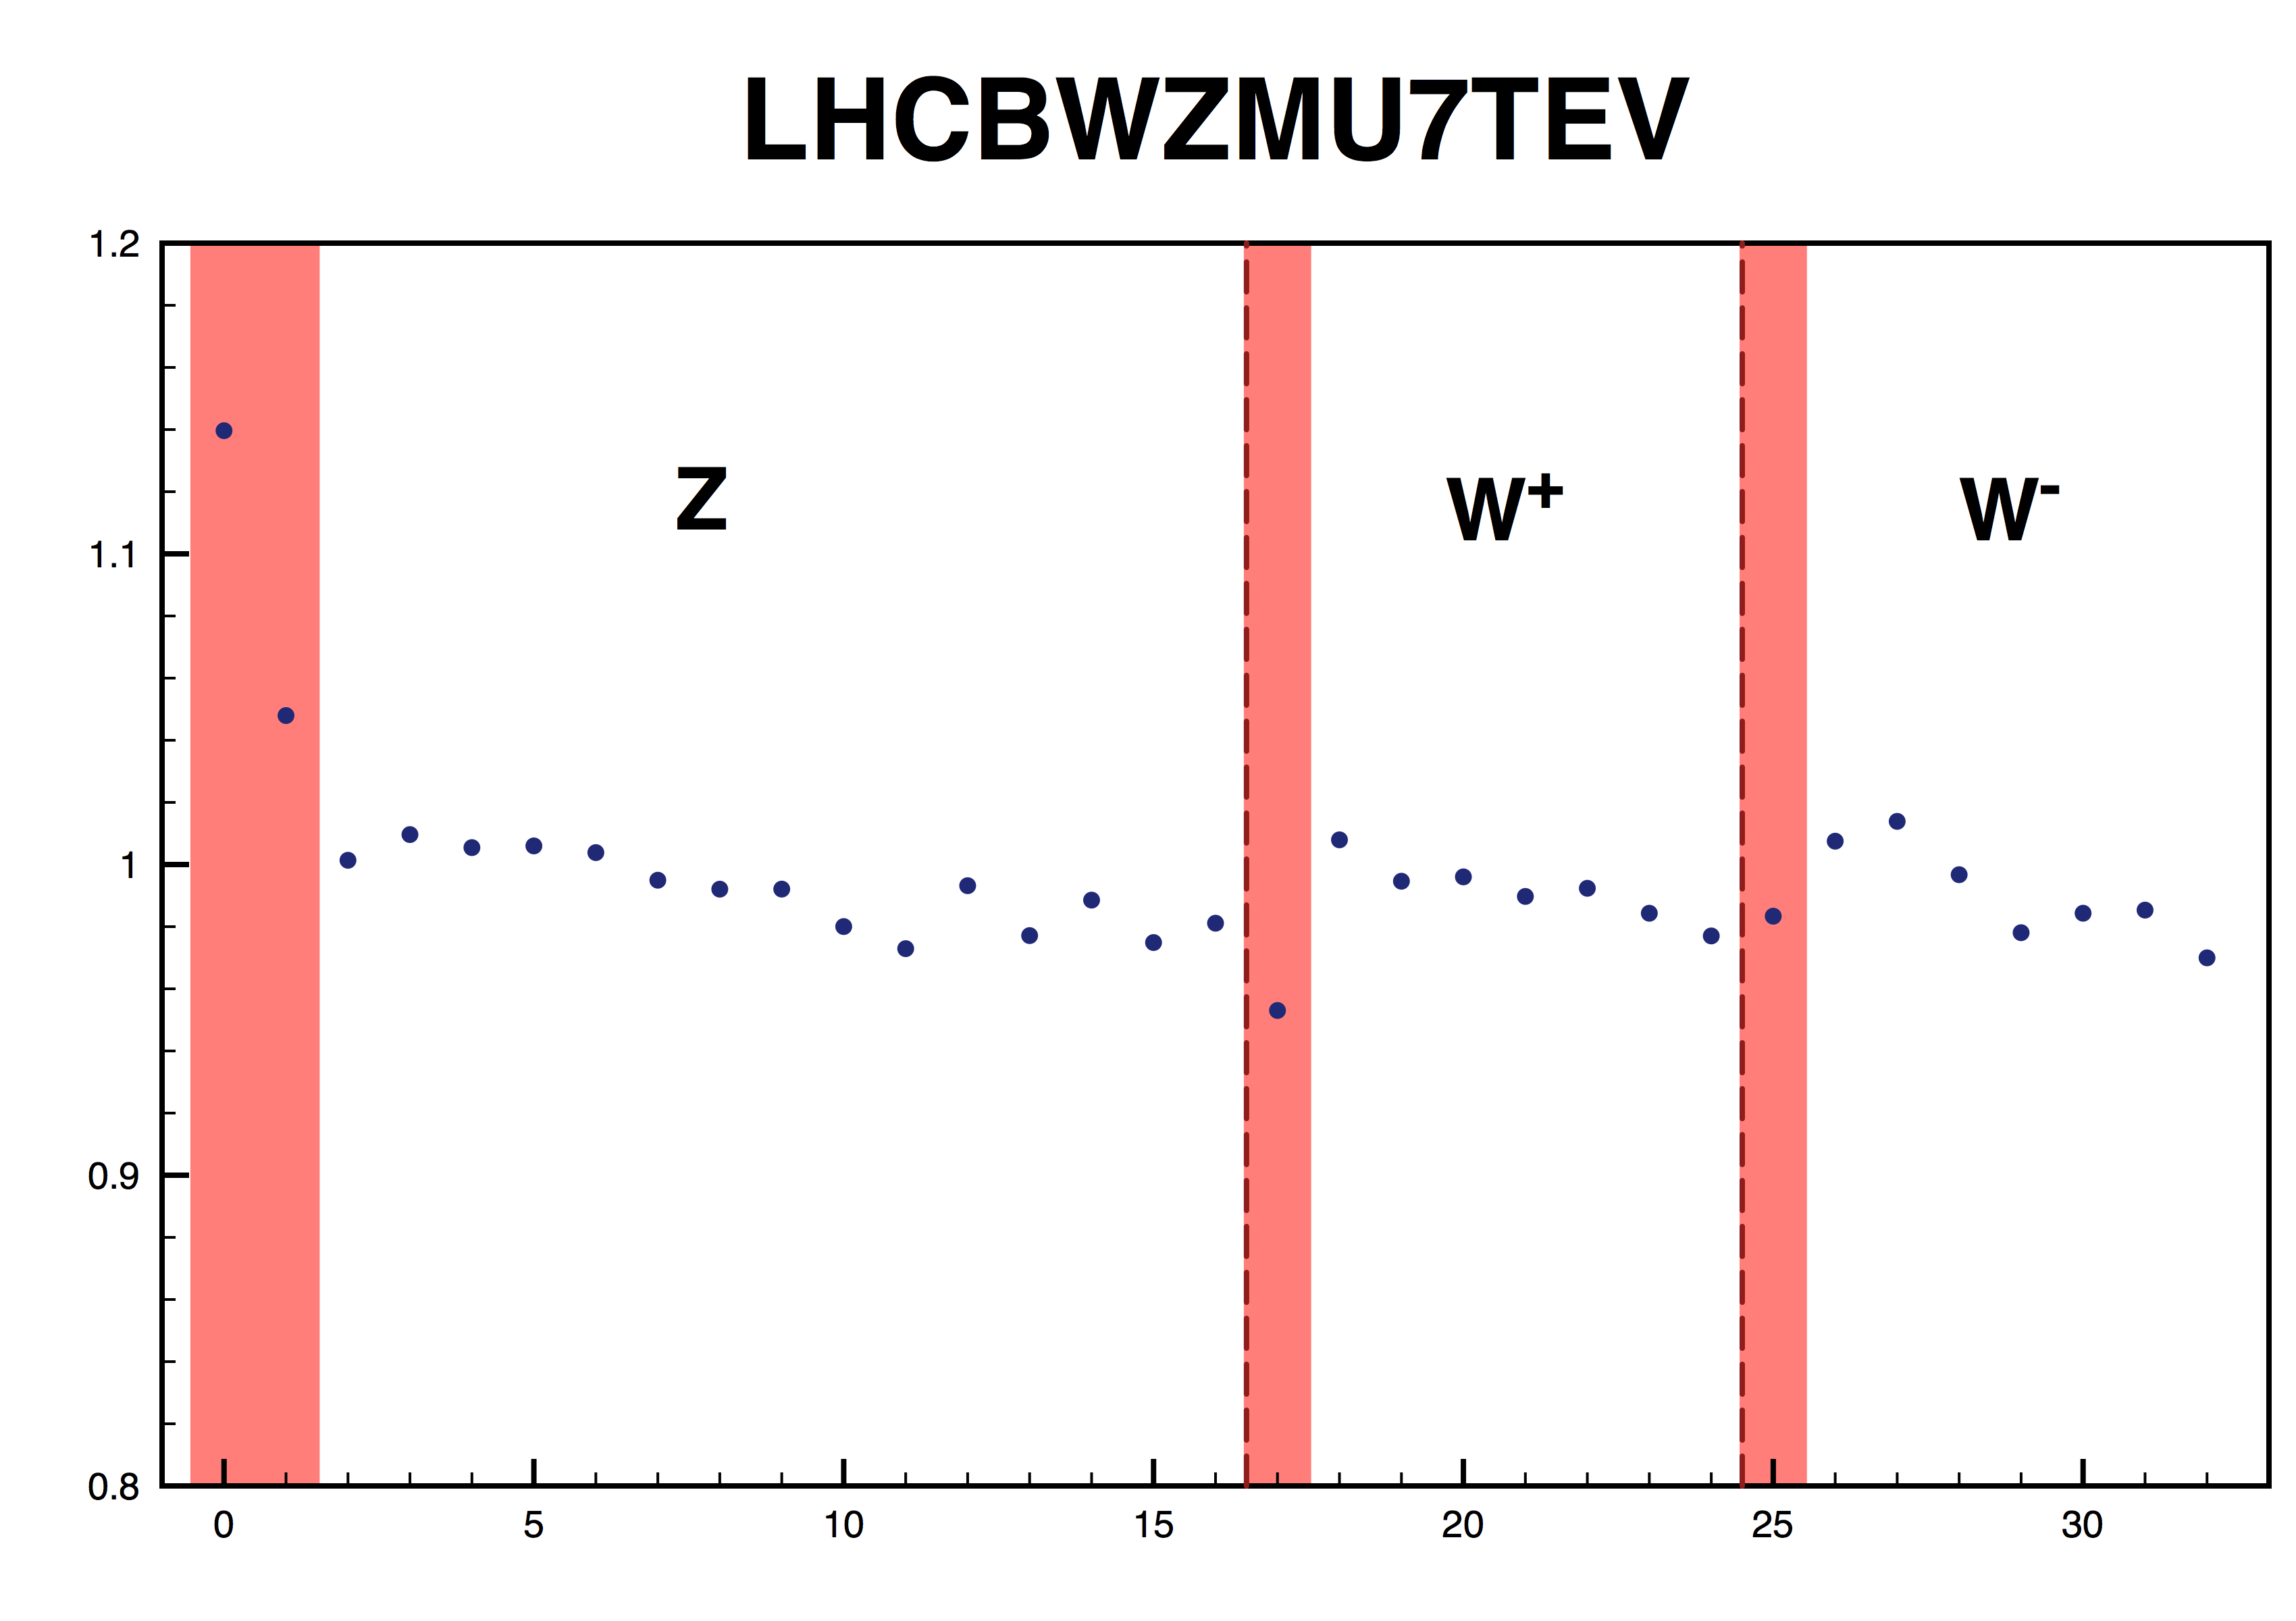
\includegraphics[width=0.49\linewidth]{images/plots/LHCBWZMU7TEV.png}
  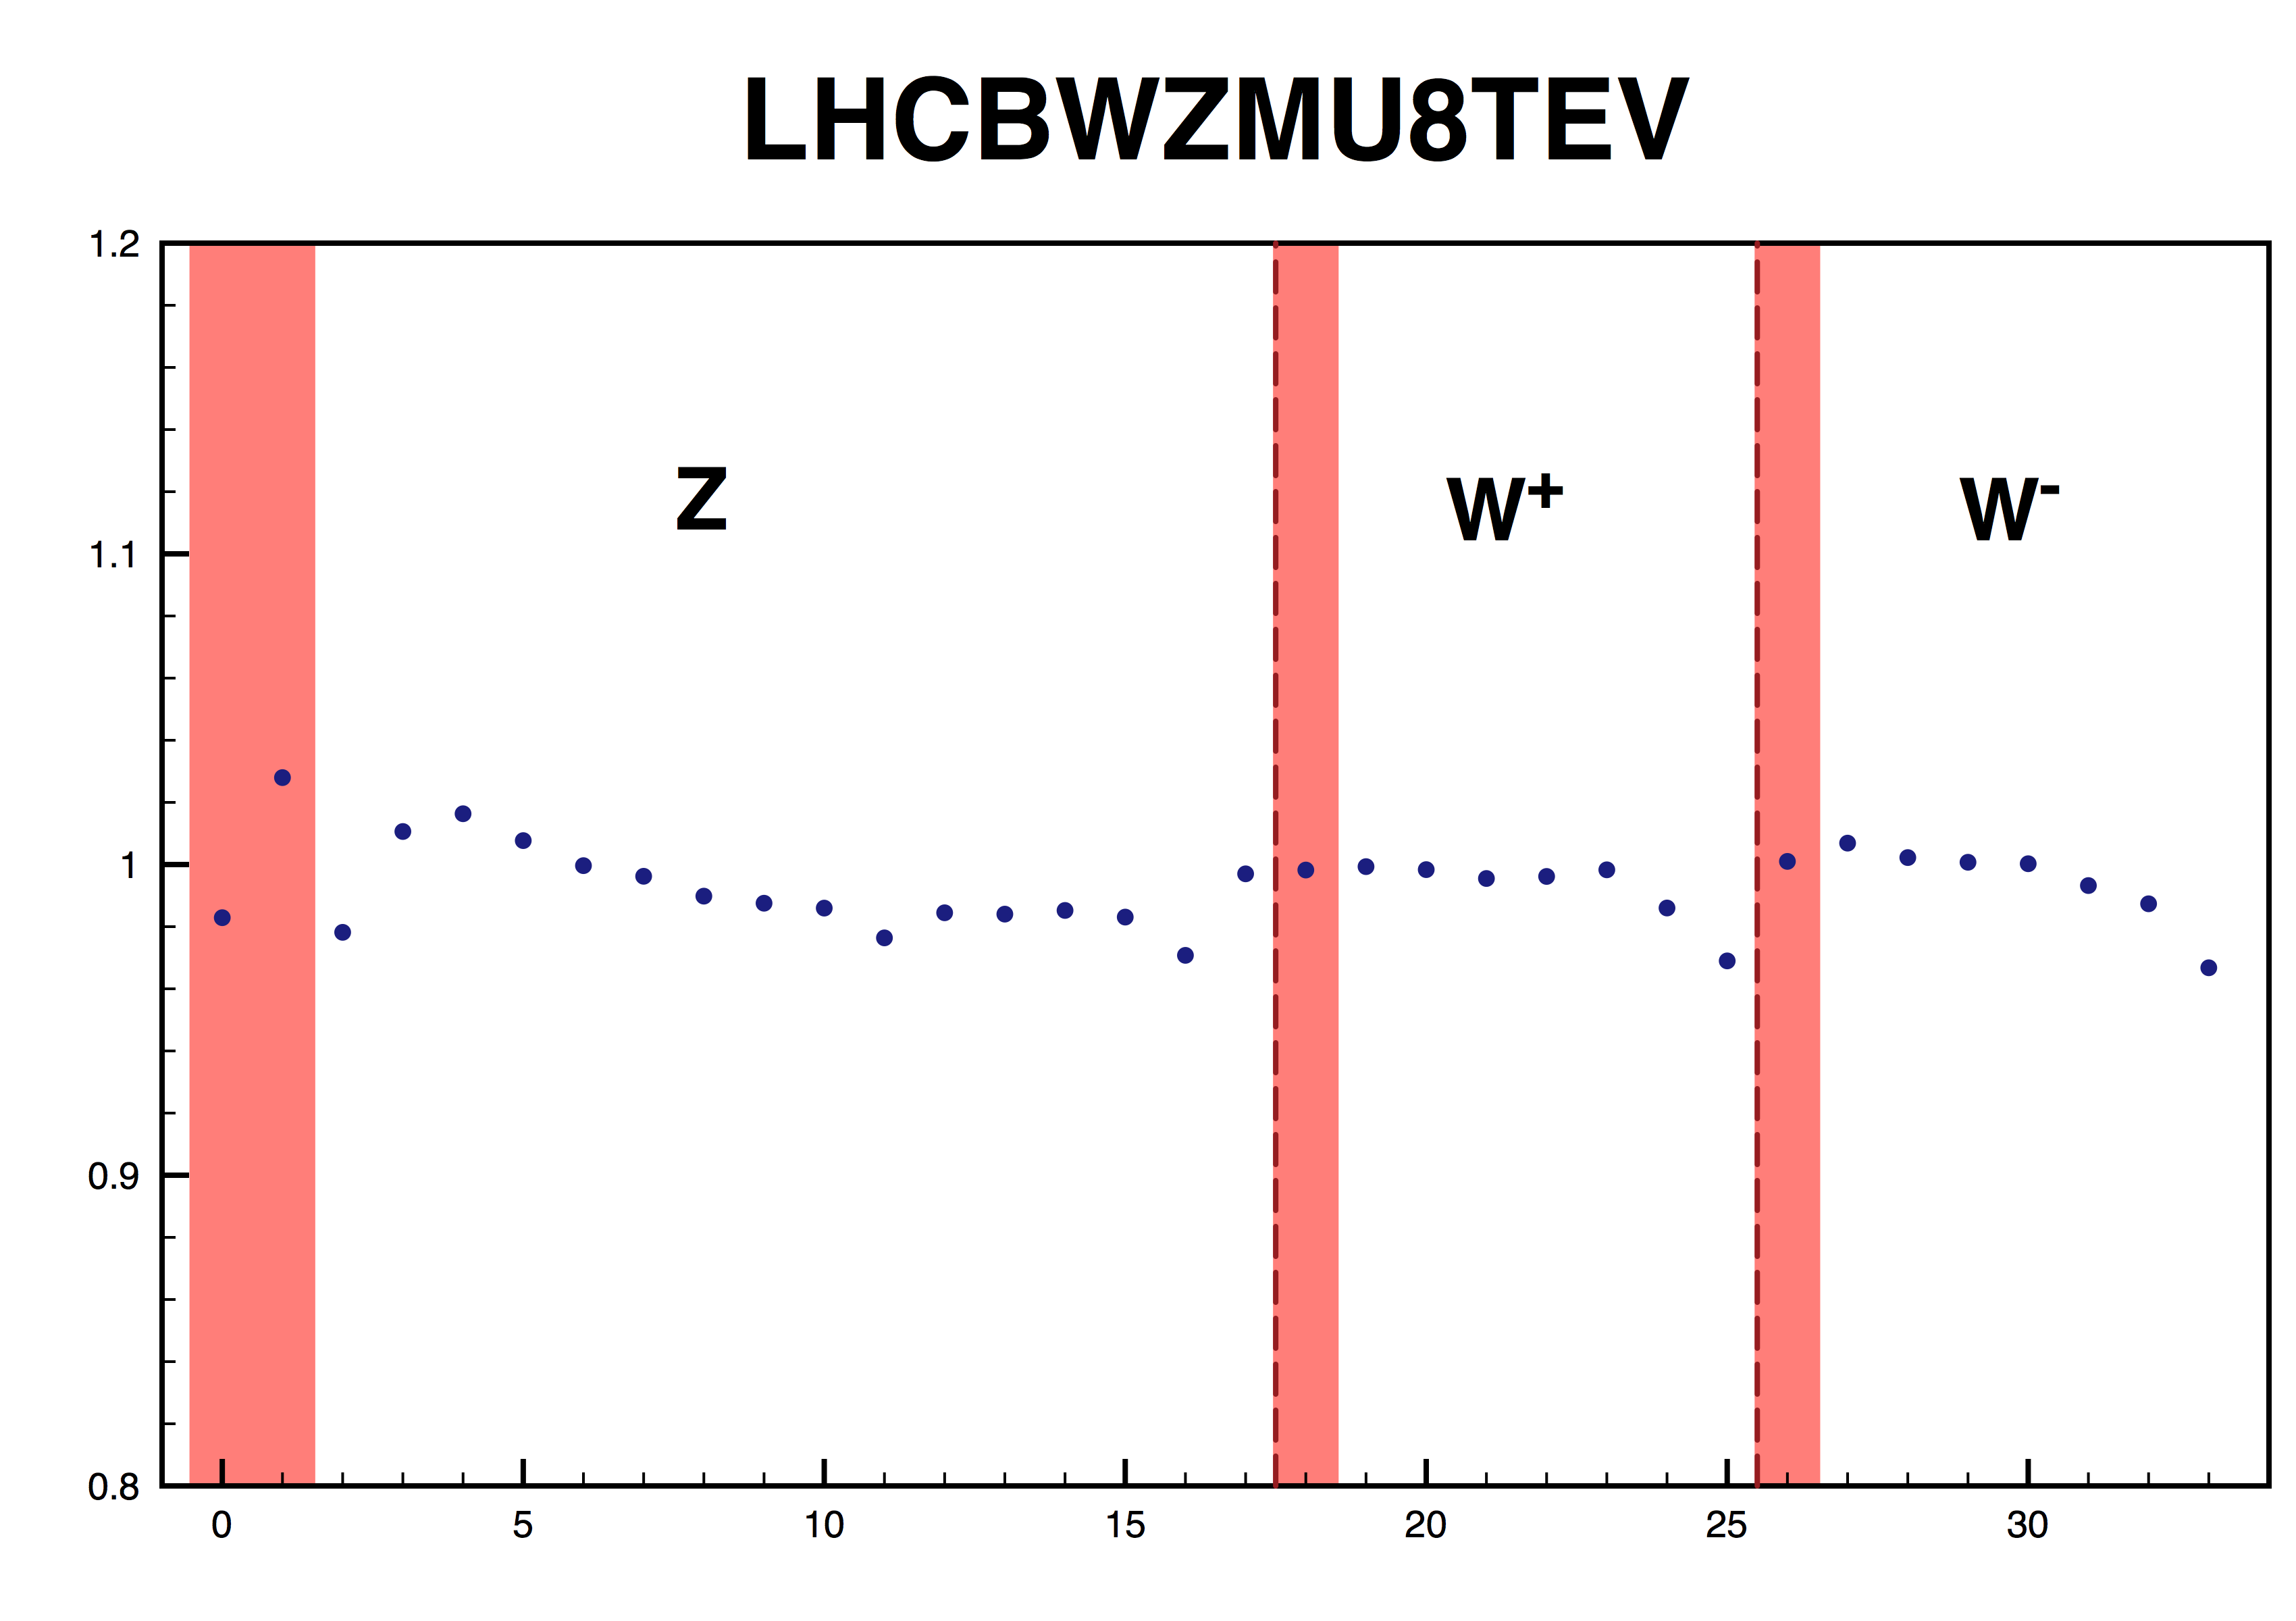
\includegraphics[width=0.49\linewidth]{images/plots/LHCBWZMU8TEV.png}
  \caption{\small   The NNLO/NLO cross-section 
    for the LHCb $7$ (left) and $8$~TeV (right) data. The central
    rapidity region which is cut is shaded in red.
    \label{fig:lhcbcf}}
\end{center}
\end{figure}
%%%%%%%%%%%%%%%%%%%%%%%%%%%%%%%%%%%%%%%%%%%%%%%%%%%%%%%%%%%
For LHCb, previous data included in NNPDF3.0 are replaced by
the final 7~TeV and 8~TeV~$W+$, $W^-$ and $Z$ rapidity distributions in the muon
channel~\cite{Aaij:2015gna,Aaij:2015zlq}. The NNLO/NLO cross-section
ratios are shown in Fig.~\ref{fig:lhcbcf}.
%
The 
Data with $|y_l|\le 2.25$ from this set have been cut because the
anomalously large size of the NNLO corrections suggests that they may
be unreliable.
Theoretical predictions are obtained at NLO using
{\tt APPLgrids} constructed using
MCFM, and at NNLO 
corrections computed using {\tt FEWZ}.



\subsection{The transverse momentum of $Z$ bosons}
\label{sec:zpt}

The transverse momentum distribution of the $Z$ boson is included for the
first time in a global PDF determination thanks to the recent computation of the process
at NNLO~\cite{Ridder:2015dxa,Ridder:2016nkl,Boughezal:2015ded,Boughezal:2016isb}.
In the NNPDF3.1 determination we include recent datasets from ATLAS and
CMS  following the detailed study in Ref.~\cite{Boughezal:2017nla}.

%

ATLAS has published measurements of the spectrum of the $Z$ 
transverse momentum 
at 7~TeV~\cite{Aad:2014xaa} and at
$8$~TeV~\cite{Aad:2015auj}. Measurements are performed
in the $Z/\gamma^*\to e^+e^-$ and $Z/\gamma^*\to \mu^+\mu^-$ 
channels which are then combined. The 7~TeV data are based
on an integrated luminosity of 4.7~${\rm fb}^{-1}$, while the 8~TeV data are
based on an integrated luminosity of 20.3~fb$^{-1}$. We now discuss each of these two datasets in
turn.

The 7~TeV data are taken at the $Z$ peak, reaching values of the $Z$
transverse momentum of up to $p_T^Z=800$ GeV.
%
They are given inclusively for $Z/\gamma^*$ rapidities up to
$|y_Z|=2.4$, as well as in three separated rapidity bins
given by $0.0\le |y_Z| \le 1.0$, $1.0 \le |y_Z| \le
2.0$ and $2.0 \le |y_Z| \le 2.4$.
%
In order to maximize the potential constraint on PDFs, only the differential
measurement will be considered.
%
The measurement is presented in terms of normalized cross-sections
$(1/\sigma_Z)\,d\sigma(Z)/d p_T^Z$, where $\sigma_Z$
is the fiducial cross-section in the corresponding di-lepton rapidity
bin.
%
%The data are characterized by rather small
%statistical and systematic uncertainties, typically below 
%1\% in all $p_T$ bins up to 150 GeV,
%for central lepton rapidities ($|y_Z|\le 2.0$), 
%increasing up to about 3\% for the
%largest rapidity bin. 
This dataset has been left out of default NNPDF3.1 dataset, for reasons to be discussed in Sect.~\ref{sec:impactzpt}.

The 8~TeV dataset, which reaches $p_T^Z$ values as high as $900$~GeV, 
is presented in three separate invariant mass bins:
low mass below the $Z$-peak, on-peak, and high mass above the $Z$-peak up to $\Mll=$ 150 GeV.
%
In addition, the measurement taken at the $Z$-peak
is provided both inclusively in the whole rapidity range
$0.0<|y_Z|<2.4$ as well as exclusively in six
separate rapidity bins $0<y_Z<0.4$,
$0.4<|y_Z|<0.8$, $0.8<|y_Z|<1.2$, $1.2<|y_Z|<1.6$, $1.6<|y_Z|<2.0$ and
$2.0<|y_Z|<2.4$.
%
Once again, here the more differential measurement will be used. 
%
In contrast to the 7~TeV data, the dataset is given both in terms of normalized and absolute distributions. 
We will use the latter, not only because of the extra information on the 
cross-section normalization, but also as problems can occur whenever
the data used to compute the normalization are provided in a range
which differs from that of the data used for PDF determination. This problem is 
discussed in detail in Ref.~\cite{Boughezal:2017nla} and described in Sect.~\ref{sec:impactzpt}.

CMS has measured the cross-sections differentially in $p_T$ and rapidity $y_Z$
at 8~TeV~\cite{Khachatryan:2015oaa}, based
on an integrated luminosity of 19.7 fb$^{-1}$ in the muon channel.
Data is provided in five rapidity bins 
 $0.0<|y_Z|<0.4$,
$0.4<|y_Z|<0.8$, $0.8<|y_Z|<1.2$, $1.2<|y_Z|<1.6$ and $1.6<|y_Z|<2.0$.
%
We do not consider a previous CMS measurement at 7~TeV~\cite{Chatrchyan:2011wt}, which
is based on a smaller dataset, and would constitute
double counting of the double differential distributions~\cite{Chatrchyan:2013tia} already included
in NNPDF3.0, and retained in NNPDF3.1.


Three sets of kinematic cuts are applied to the data. 
%
Firstly, ensuring the reliability of fixed-order perturbation theory
imposes a cut of $p_T^Z \ge$ 30 GeV
(resummation would be required for smaller $p_T$)~\cite{Boughezal:2017nla}.
%
Secondly, removing regions in which electroweak corrections
are large and comparable to the experimental data imposes
a cut of $p_T^Z \le 150~(170)$ GeV for the ATLAS~(CMS)
data~\cite{Boughezal:2017nla}.  
%
Finally, the CMS dataset in the largest rapidity bin is discarded
due to an apparent incompatibility with both the corresponding ATLAS
measurement in the same bin and the theoretical prediction. The origin of this incompatibility
remains unclear~\cite{Boughezal:2017nla}.

Theoretical predictions have been obtained from
Ref.~\cite{Boughezal:2017nla}, based upon the NNLO computation of
$Z$+jet production of Refs.~\cite{Boughezal:2015ded,Boughezal:2016isb}.
Factorization and renormalization scales are chosen as
\be
\mu_R=\mu_F =
\sqrt{(p_T)^2+\Mll^2} \, ,
\ee
where $\Mll$ is the invariant mass of the
final-state lepton pair.
%
The calculation includes the $Z$ and $\gamma^*$ contributions, their interference and decay to
lepton pairs. The NNLO/NLO ratio is shown in
Fig.~\ref{fig:zptcf} for the observables with the ATLAS and CMS acceptance cuts, 
computed using NNPDF3.0 PDFs, with
$\alpha_s(m_Z)=0.118$; the NNLO correction varies
from around
2-3\% at low $p_T$ up to around 10\% at high $p_T$ and is therefore
required in order to describe data with sub-percent accuracy. 
% 

%%%%%%%%%%%%%%%%%%%%%%%%%%%%%%%%%%%%%%%%%%%%%%%%%%%%%%%%%%%%%%%%
\begin{figure}[t]
\begin{center}
  \includegraphics[width=0.49\linewidth]{images/plots/atlas7tev_CF.pdf}
  \includegraphics[width=0.49\linewidth]{images/plots/cms8tev_CF.pdf}\\
  \includegraphics[width=0.49\linewidth]{images/plots/atlas8tevy_CF.pdf}
  \includegraphics[width=0.49\linewidth]{images/plots/atlas8tevm_CF.pdf}
  \caption{\small   The NNLO/NLO cross-section 
    for the $Z$ $p_T$ data
    corresponding
    to the acceptance cuts and binning
    of the ATLAS 7~TeV (top left), CMS 8~TeV (top right),
    and the ATLAS 8 TeV (bottom) rapidity (left) and invariant mass
    (right) distributions.
    \label{fig:zptcf}}
\end{center}
\end{figure}
%%%%%%%%%%%%%%%%%%%%%%%%%%%%%%%%%%%%%%%%%%%%%%%%%%%%%%%%%%%

Even the most accurate results for the NNLO/NLO correction factor
still display fluctuations, as shown in Fig.~\ref{fig:zptcf} where we
plot the NNLO/NLO cross-section ratio for the central rapidity bin of
the $8$~TeV ATLAS data. The points are shown together with their
nominal Monte Carlo integration uncertainty~\cite{Boughezal:2017nla}.
The point-to-point statistical fluctuation of the theoretical prediction appears
to be larger than the typical uncorrelated statistical uncertainty on
the ATLAS dataset, which is typically at the sub-percent or even permille
level. In order to check this, we have  fitted 
 an ensemble of neural networks to the
cross-section ratio, as a function of $p_T^Z$ for fixed rapidity. 
The fit has been
performed in each of the rapidity bins for the ATLAS and CMS data; 
more details are given in Ref.~\cite{Carrazza:2017bjw}.
The result of the fit
and its one-sigma 
uncertainty are  shown in Fig.~\ref{fig:cf-zpt-fit} for the central
rapidity bin of the ATLAS data.  

 The one-sigma uncertainty of the  fit, which is determined by the
 point-to-point 
fluctuation of the NNLO computation, is at the percent level, which is
  rather larger than the
statistical uncertainty of the data. Indeed, 
it is clear by inspection of
Figs.~\ref{fig:zptcf}-\ref{fig:cf-zpt-fit} that the point-to-point fluctuations of the NNLO/NLO ratio are much larger than those
of the data themselves (as seen in
Ref.s~\cite{Aad:2014xaa},\cite{Boughezal:2017nla}). We  conclude that
there is a 
residual theoretical uncertainty on the NNLO prediction which we
estimate to be of order of 1\% for all datasets. This conclusion has
been validated and cross-checked by repeating the fit with cuts or
different functional forms. We have therefore added an extra 1\% fully
uncorrelated theoretical uncertainty to this dataset (see also Ref.~\cite{Boughezal:2017nla}).

%%%%%%%%%%%%%%%%%%%%%%%%%%%%%%%%%%%%%%%%%%%%%%%%%%%%%%%%%%%%%%%%
\begin{figure}[t]
\begin{center}
  \includegraphics[scale=0.55]{images/plots/cf-zpt-fit.pdf}
  \caption{\small
    The NNLO/NLO cross-section ratio in  
 the central rapidity bin of the 8~TeV ATLAS $Z$ $p_T$
    distribution. The result of a fit and its associate uncertainty
    are also shown.
\label{fig:cf-zpt-fit}}
\end{center}
\end{figure}
%%%%%%%%%%%%%%%%%%%%%%%%%%%%%%%%%%%%%%%%%%%%%%%%%%%%%%%%%%%

\subsection{Differential distributions and total
  cross-sections in $t\bar{t}$ production}
\label{sec:topdata}

Differential distributions for top pair production have been
included in NNPDF3.1 following the detailed study of Ref.~\cite{Czakon:2016olj}.
ATLAS and CMS have performed measurements of these distributions with a
variety of choices of kinematic variables, including the top quark rapidity
$y_t$, the rapidity of the top pair $y_{t\bar{t}}$, the transverse 
momentum of the top quark $p_T^t$, and the invariant mass of the top-antitop
system $m_{t\bar{t}}$. For ATLAS both absolute and normalized 
differential distributions are provided, whereas CMS only provides
normalized results.
%
Perturbative QCD corrections for all these distributions have been 
computed at NNLO~\cite{Czakon:2015owf,Czakon:2016dgf}.
%
In order to avoid double counting, only one distribution per
experiment can be included in the dataset, as the statistical correlations
between different distributions are not available.
%
The choice of differential distributions adopted in NNPDF3.1 follows the 
recommendation of Ref.~\cite{Czakon:2016olj}, where
a comprehensive study of the impact on the gluon PDF of 
various combinations of differential top pair distributions was performed. 
%
It was found that the normalized rapidity distributions have the
largest constraining power and lead to a good agreement between theory and data
for ATLAS and CMS.
%
The use of rapidity distributions has some further  advantages.
%
First, it reduces the risk of possible contamination by BSM effects.
%
For example, heavy resonances would be kinematically suppressed
in the rapidity distributions, but not in the tails of the $m_{t\bar{t}}$ and 
$p_T^t$ distributions.
%
Second, rapidity distributions exhibit a milder sensitivity upon variations 
of the value of $m_t$ than the $p_T^t$ and $m_{t\bar{t}}$ 
distributions~\cite{Czakon:2016vfr}.

We therefore include the $8$~TeV normalized
rapidity distributions in the lepton+jets final
state from ATLAS~\cite{Aad:2015mbv} and 
CMS~\cite{Khachatryan:2015oqa}, which 
correspond respectively to an integrated
luminosity of $20.3$ fb$^{-1}$ and $19.7$ fb$^{-1}$. 
%
We consider measurements in the full phase space, with observables 
reconstructed in terms of the top or top-pair kinematic variables, because
NNLO results are available only for stable top quarks.
We also include, again following Ref.\cite{Czakon:2016olj},
the most recent total cross-sections measurements at $7$, $8$ and $13$~TeV from
ATLAS~\cite{Aad:2014kva,Aaboud:2016pbd} and
CMS~\cite{Khachatryan:2016mqs,CMS:2016syx}.
%
They replace previous measurements from 
ATLAS~\cite{ATLAS:2012aa,ATLAS:2011xha,TheATLAScollaboration:2013dja}
and CMS~\cite{Chatrchyan:2013faa,Chatrchyan:2012bra,Chatrchyan:2012ria} 
included in NNPDF3.0. 

At NLO theoretical predictions have been generated with {\tt Sherpa}~\cite{Gleisberg:2008ta}, in a format 
compliant to {\tt APPLgrid}~\cite{Carli:2010rw}, using
the {\tt MCgrid} 
code~\cite{DelDebbio:2013kxa} and the {\tt Rivet}~\cite{Buckley:2010ar} 
analysis package, with {\tt OpenLoops}~\cite{Cascioli:2011va} for the NLO 
matrix elements. 
%
All calculations have been performed with large Monte Carlo integration 
statistics in order to ensure that residual numerical fluctuations are 
negligible.
%
Our results have been carefully benchmarked against those obtained from 
the code of~\cite{Czakon:2016dgf}.
%
Renormalization and factorization scales, $\mu_R$ and $\mu_F$
respectively, have 
been chosen based on the recommendation of Ref.~\cite{Czakon:2016dgf} as
\be
\label{eq:scale1}
\mu_R=\mu_F=\mu=H_T/4 \, , \qquad H_T \equiv \sqrt{m_t^2+\lp {p_T^t}\rp^2}
+ \sqrt{m_t^2+\lp {p_T^{\bar{t}}}\rp^2} \, ,
\ee
where $m_t=173.3$ GeV is the PDG world average for the
top-quark pole mass~\cite{Agashe:2014kda},
and $p_T^t$ ($p_T^{\bar{t}}$) is the top (anti-top) transverse momentum.
NLO theoretical predictions for normalized differential distributions have been obtained
by dividing their absolute counterparts by the cross-section
integrated over the kinematic range of the data.


The NNLO correction factors have been computed separately
for the absolute  differential cross-sections and their normalizing total cross-sections. 
%
Differential cross-sections have been determined using the 
code of~\cite{Czakon:2016dgf}, with the scale choice Eq.~(\ref{eq:scale1}).
%
Results for the NNLO/NLO ratio are shown in
Fig.~\ref{fig:ttbar-cfact}, where it can be seen that the size of the
NNLO corrections is $6\%$ and $9\%$, actually smaller
than the data uncertainty, with a reasonably flat shape in the kinematic
region covered by the data.
We also show explicitly the dependence of the results on the PDF set
used in the calculation by using three different global PDF sets: it
is clear that this dependence is completely negligible.

Total cross-sections have been computed with the {\tt top++}
code~\cite{Czakon:2011xx} at NNLO+NNLL, and with fixed scales
$\mu_R=\mu_F=m_t$, following the recommendation of
Ref.~\cite{Czakon:2016dgf} which suggests that NNLO+NNLL resummed
cross-sections should be used in conjunction to NNLO differential
distributions if the latter are determined using a dynamical scale choice.


%

%%%%%%%%%%%%%%%%%%%%%%%%%%%%%%%%%%%%%%%%%%%%%%%%%%%%%%%%%%%%%%%%
\begin{figure}[t]
\begin{center}
  \includegraphics[scale=0.31,angle=270]{images/plots/ttbar-cfact_yt.pdf}
  \includegraphics[scale=0.31,angle=270]{images/plots/ttbar-cfact_ytt.pdf}\\
  \caption{\small
    The NNLO/NLO cross-section ratio for the top quark rapidity $y_t$
    (left)
    and top-quark pair rapidity $y_{t\bar{t}}$ (right) corresponding
    to the 8~TeV ATLAS and CMS data.
    %
     Results obtained with three different input PDF sets, NNPDF3.0,
     CT14, and MMHT14, are shown.
\label{fig:ttbar-cfact}}
\end{center}
\end{figure}
%%%%%%%%%%%%%%%%%%%%%%%%%%%%%%%%%%%%%%%%%%%%%%%%%%%%%%%%%%%





%%%%%%%%%%%%%%%%%%%%%%%%%%%%%%%%%%%%%%%%%%%%%%%%%%%%%%%%%%%%%%%%%%%%%%%%%%%%%%%%%%%%%%%%%%
%%%%%%%%%%%%%%%%%%%%%%%%%%%%%%%%%%%%%%%%%%%%%%%%%%%%%%%%%%%%%%%%%%%%%%%%%%%%%%%%%%%%%%%%%%
%%%%%%%%%%%%%%%%%%%%%%%%%%%%%%%%%%%%%%%%%%%%%%%%%%%%%%%%%%%%%%%%%%%%%%%%%%%%%%%%%%%%%%%%%
%
